\documentclass[10pt]{scrartcl}

%Math
\usepackage{amsmath}
\usepackage{amsfonts}
\usepackage{amssymb}
\usepackage{amsthm}
\usepackage{ulem}
\usepackage{stmaryrd} %f\UTF{00FC}r Blitz!

%PageStyle
\usepackage[ngerman]{babel} % deutsche Silbentrennung
\usepackage[utf8]{inputenc} 
\usepackage{fancyhdr, graphicx}
\usepackage[scaled=0.92]{helvet}
\usepackage{enumitem}
\usepackage{parskip}
\usepackage[a4paper,top=2cm]{geometry}
\setlength{\textwidth}{17cm}
\setlength{\oddsidemargin}{-0.5cm}
\usepackage[scaled=0.92]{helvet}
\usepackage{lastpage} % for getting last page number
\renewcommand{\familydefault}{\sfdefault}
\usepackage{wrapfig}


% Shortcommands
\newcommand{\Bold}[1]{\textbf{#1}} %Boldface
\newcommand{\Kursiv}[1]{\textit{#1}} %Italic
\newcommand{\T}[1]{\text{#1}} %Textmode
\newcommand{\Nicht}[1]{\T{\sout{$ #1 $}}} %Streicht Shit durch

%Arrows
\newcommand{\lra}{\leftrightarrow} 
\newcommand{\ra}{\rightarrow}
\newcommand{\la}{\leftarrow}
\newcommand{\lral}{\longleftrightarrow}
\newcommand{\ral}{\longrightarrow}
\newcommand{\lal}{\longleftarrow}
\newcommand{\Lra}{\Leftrightarrow}
\newcommand{\Ra}{\Rightarrow}
\newcommand{\La}{\Leftarrow}
\newcommand{\Lral}{\Longleftrightarrow}
\newcommand{\Ral}{\Longrightarrow}
\newcommand{\Lal}{\Longleftarrow}

% Code listenings
\usepackage{color}
\usepackage{xcolor}
\usepackage{listings}
\usepackage{caption}
\DeclareCaptionFont{white}{\color{white}}
\DeclareCaptionFormat{listing}{\colorbox{gray}{\parbox{\textwidth}{#1#2#3}}}
\captionsetup[lstlisting]{format=listing,labelfont=white,textfont=white}
\lstdefinestyle{JavaStyle}{
 language=Java,
 basicstyle=\footnotesize\ttfamily, % Standardschrift
 numbers=left,               % Ort der Zeilennummern
 numberstyle=\tiny,          % Stil der Zeilennummern
 stepnumber=5,              % Abstand zwischen den Zeilennummern
 numbersep=5pt,              % Abstand der Nummern zum Text
 tabsize=2,                  % Groesse von Tabs
 extendedchars=true,         %
 breaklines=true,            % Zeilen werden Umgebrochen
 frame=b,         
 %commentstyle=\itshape\color{LightLime}, Was isch das? O_o
 %keywordstyle=\bfseries\color{DarkPurple}, und das O_o
 basicstyle=\footnotesize\ttfamily,
 stringstyle=\color[RGB]{42,0,255}\ttfamily, % Farbe der String
 keywordstyle=\color[RGB]{127,0,85}\ttfamily, % Farbe der Keywords
 commentstyle=\color[RGB]{63,127,95}\ttfamily, % Farbe des Kommentars
 showspaces=false,           % Leerzeichen anzeigen ?
 showtabs=false,             % Tabs anzeigen ?
 xleftmargin=17pt,
 framexleftmargin=17pt,
 framexrightmargin=5pt,
 framexbottommargin=4pt,
 showstringspaces=false      % Leerzeichen in Strings anzeigen ?        
}

 
\fancypagestyle{firststyle}{ %Style of the first page
\fancyhf{}
\fancyheadoffset[L]{0.6cm}
\lhead{

\includegraphics[scale=0.8]{./img/fhnw_logo_en.png}}
\renewcommand{\headrulewidth}{0pt}
\lfoot{school of business,\linebreak www.fhnw.ch }
}

\fancypagestyle{documentstyle}{ %Style of the rest of the document
\fancyhf{}
\fancyheadoffset[L]{0.6cm}
\lhead{

\includegraphics[scale=0.8]{./img/fhnw_logo_en.png}}
\renewcommand{\headrulewidth}{0pt}
\lfoot{\thepage\ / \pageref{LastPage} }
}

\pagestyle{firststyle} %different look of first page
 
\title{ %Titel
Volkswirtschaftslehre
\vspace{0.2cm}
\Large (Zusammenfassung)}

 \begin{document}
 \maketitle
 \thispagestyle{firststyle}
 \pagestyle{firststyle}
 \begin{abstract}
 \begin{center}
  Zusammenfassung des Modul VWL (HS14) von Fabian Stebler. 
 \end{center}
 \vspace{0.5cm}
\hrulefill
\end{abstract}

 \pagestyle{documentstyle}
 \tableofcontents
 \pagebreak

\section{Begriffe}
\subsection{Datenarten}
\begin{itemize}
\item {\bf Strukturierte Daten } folgen einer bestimmten Struktur. {\it z.B. Verkaufsdaten, Patientendaten, Produktdaten}
\item {\bf Unstrukturierte Daten} sind meistens Text und Bilder und folgen keiner Struktur.
\item {\bf Semistrukturierte Daten} sind eine Kombination der zwei oben genannten Arten {\it z.B. Kataloge, Akten}
\end{itemize}
\subsection{Datenverwaltung}
\begin{itemize}
\item Daten müssen persistent auf einem Datenträger gespeichert werden
\item Daten müssen eingegeben, verändert und gelöscht werden können (von autorisierten Personen)
\item Daten müssen abgefragt werden können
\item Die Struktur der Daten (Kontext) muss definiert werden können; bei der Eingabe muss kontrolliert werden, dass die Daten diese Struktur folgen
\item Menge der Daten, Komplexität der Daten, Anzahl Benutzer sind kein Hindernis
\end{itemize}
\subsection{Datenbank}
\begin{itemize}
\item ist eine logische zusammenhängende Sammlung von Daten, die einen Ausschnitt der realen Welt ( Miniwelt ) beschreiben
\item ist keine zufällige Datensammlung
\item wird für einen bestimmten Zweck entworfen, entwickelt und mit Daten gefüllt
\item ist dauerhaft verfügbar („Persistenz“)
\item kann jede beliebige Grösse und Komplexität aufweisen
\item widerspiegelt Änderungen der Miniwelt
\item ist mehrfachbenutzbar („parallel zugreifbar“)
\item weisst eine hohe „Datenqualität“ auf (Daten sind konsistent)
\item erlaubt eine bequeme – flexible – effiziente Handbarkeit von Daten
\end{itemize}

\subsection{Datenbankverwaltungs- /Datenbankmanagementsystem (DBMS)}
Ein DBMS ist ein Softwaresystem, welches die {\bf Definition, Konstruktion} und {\bf Manipulation} von Datenbanken für verschiedene Anwendugen unterstützt.
\begin{itemize}
\item {\bf Definition} einer Datenbank: Spezifikation der Struktur der in der Datenbank zu speichernden Daten (Datenbankentwurf)
\item {\bf Konstruktion} der Datenbank: Speicherung der Daten (Dateneingabe)
\item {\bf Manipulation} einer Datenbank: Anfragen der Datenbank, Aktualisierung der Datenbank
\end{itemize}
\subsection{Datenbanksystem (DBS)}
Ein DBS umfasst eine Datenbank und ein Datenbankmanagementsystem. {\it (z.B.: Krankenhausverwaltungssystem, Hochschuldatenbank)}
\subsection{Datenmodell}
\begin{itemize}
\item eine Sammlung von Konzepten, die benutzt werden um die Struktur der
Datenbank zu beschreiben. (Basis für die Datenabstraktion)
\item eine Reihe von Basisoperationen für die Spezifikation von Anfragen und die
Aktualisierung der Datenbank
\end{itemize}
\subsubsection{Kategorisierung der Datenmodelle}
entsprechend der Konzepte für die Beschreibung der Daten:
\begin{itemize}
\item[] {\bf konzeptuelle Datenmodelle}(„höhere“, “semantische“)\\
{\it Bsp: Entity Relationship Model (ER-Modell), Unified Modelling Language(UML)}
\begin{itemize}
\item anwendungsnah
\item systemunabhängig
\end{itemize} 
\item[] {\bf logische Datenmodelle}\\
{\it Bsp: relationales Datenmodell, objektorientiertes Datenmodell,
Netzwerkdatenmodell, hierarchisches Datenmodell}
\begin{itemize}
\item Schnittstelle von DBMS
\end{itemize} 
\item[] {\bf physische Datenmodelle} ("niedere", "interne")\\
{\it Beschreibung von Details der Datenspeicherung (gerätenah, nur für Spezialisten -- wenn überhaupt --zugänglich}
\end{itemize}

\subsection{Datenbankschema}
die Beschreibung der Datenbank.
\begin{itemize}
\item welche Struktur ist für eine DB gewünscht?
\item wird im Verlauf des Datenbankentwurfs spezifiziert mittels der vom Datenmodell angebotenen Konzepten
\end{itemize}


\subsection{Datenbanksprachen}
\begin{itemize}
\item {\bf Data Definition Language (DDL } wird für die Definition vom DB-Schema eingesetzt.
\item {\bf Data Manipulation Language (DML)}
\begin{itemize}
\item erlaubt den Zugriff auf die Datenbank (anfragen oder aktualisieren)
\item prozedural (wie?), deskriptiv (was?)
\item kann selbständig (Anfragesprache) oder Teilsprache (in „host language“
eingebettet) sein
\end{itemize}
\item {\bf Storage Definition Language (SDL)} wird für die Definition der internen Speicherungsstrukturen eingesetzt.
\end{itemize}
\subsection{Betrieb von Datenbanksystemen}
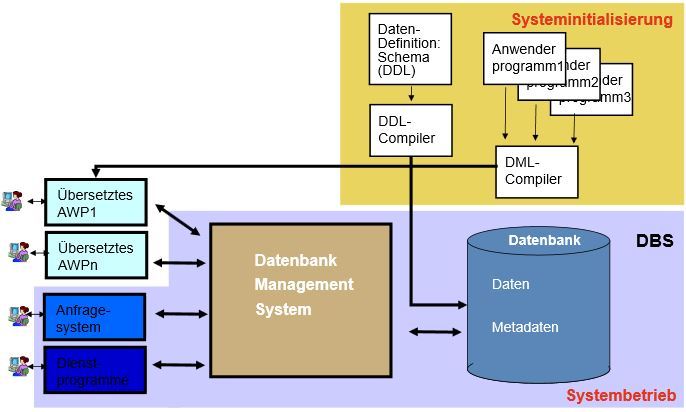
\includegraphics[width=1\textwidth]{img/betrieb-dbs.jpg}

\subsection{Systemarchitektur}




\begin{wrapfigure}{L}{0.4\textwidth}
  \begin{center}
    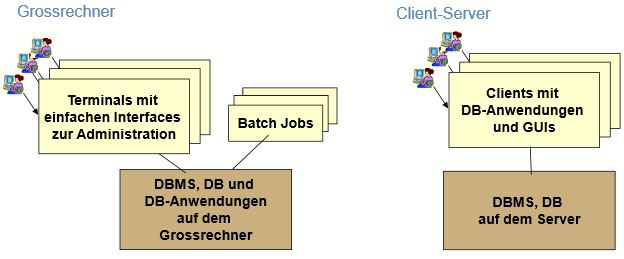
\includegraphics[width=0.4\textwidth]{img/sysarc-1.jpg}
  \end{center}
Vorteile Client-Server:
\begin{itemize}
\item Skalierbarkeit: Clientrechner übernehmen einen Teil der Last - je mehr Nutzer desto mehr Clientrechner.
\item Verfügbarkeit: Hardware am Server kann redundant ausgelegt werden
\item Sicherheit: Server und Zugang zum Server sind beschützt
\item Administration: Backups nur am Server
\end{itemize}
\end{wrapfigure}


\begin{wrapfigure}{R}{0.4\textwidth}
  \begin{center}
    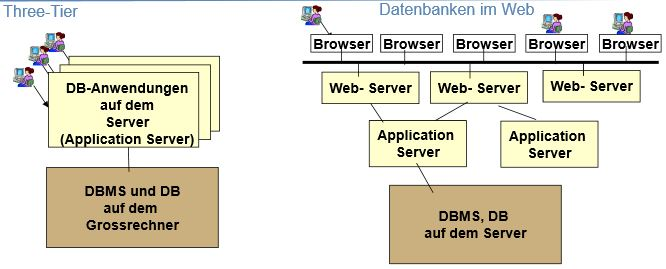
\includegraphics[width=0.4\textwidth]{img/sysarc-2.jpg}
  \end{center}
Vorteile Multi-Tier:
\begin{itemize}
\item Architektur: Schichtenarchitektur (a) Jede Ebene implementiert einen anderen Aspekt wie Datenbank, Anwendungen, GUI, ...) und (b) man kann unterschiedliche Anbieter für einzelnen Schichten haben wie Oracle für die Datenbank, Apache für den Webserver, Microsoft fürs GUI
\item Jede Schicht kann auf einem eigenen Rechner implementiert werden. Es können aber auch mehrere Schichten auf einem Rechner installiert werden.
\item Skalierbarkeit auf jeder Schicht bis auf Datenbank
\end{itemize}
\end{wrapfigure}



 \end{document}